 \documentclass[11pt,a4paper,final]{report}
\usepackage[utf8]{inputenc}
\usepackage{amsmath}
\usepackage{amsfonts}
\usepackage{amssymb}
\usepackage{graphicx}
\usepackage{geometry}
\usepackage{caption}
\usepackage{float}
\usepackage{subcaption}
\geometry{
 a4paper,
 total={170mm,257mm},
 left=20mm,
 top=12mm,
}

\setcounter{secnumdepth}{4}
\setcounter{tocdepth}{4}
 
\def\thesection{\arabic{section}}

\setlength{\jot}{5pt}

\newcommand{\ZZ}{$ZZ\to ll\nu\nu$ }
\newcommand{\Zgam}{$Z\gamma\to ll\gamma$ }

\renewcommand{\arraystretch}{1.2}
\usepackage{hyperref}

\begin{document}
\begin{titlepage}
\centering
\vfill
\vfill

\includegraphics[width = \linewidth]{Title_Head.png}
\vspace{1 in}\\
{\huge Estimation of $ZZ \rightarrow ll\nu\nu$ background using $Z(\rightarrow ll)+\gamma$ data}
\vfill
{\LARGE\textbf{Mid Year Report - November 2017}}
\vfill
{\Large Submitted to\\ Indian Institute of Science Education and Research, Pune\\in partial fulfilment of the requirements of the\\ \vspace{0.15cm}BS-MS Dual Degree Programme}
\vfill
{\Large by}
\vfill
{\Large Mangesh Sonawane\\Registration Number: 20131083\\}
\vfill
{\Large June 2017 - May 2018\\}
{\Large Supervisor: Dr. Beate Heinemann\\}
{\Large Conducted at DESY, Hamburg\\\vspace{0.15cm}Notkestra{\ss}e 85, 22607}
\vfill
\vfill
\end{titlepage}
\newpage
\vfill
\begin{center}
\textbf{\LARGE CERTIFICATE}
\end{center}
This is to certify that this report, entitled "\textit{Estimation of $ZZ \to ll\nu\nu$ background using $Z(\to ll)+\gamma$ data}" towards the partial fulfilment of the BS-MS dual degree programme at the Indian Institute of Science Education and Research, Pune, represents study/work carried out by Mangesh Sonawane at The Deutsches Elektronen-Synchrotron (DESY), Hamburg, under the supervision of Dr. Beate Heinemann, Professor, experimental Particle Physics, Department of Physics at the Albert-Ludwigs-Universit{\"a}t, Freiburg, and is submitted for Mid-Year Evaluation in November 2017, during the academic year 2017-2018.
\vfill
Mangesh Sonawane \hfill Dr. Beate Heinemann
\vfill
{\noindent}Committee:\\
Dr. Beate Heinemann\\
Dr. Seema Sharma
\vfill
\newpage
\tableofcontents
\newpage
\section*{Abstract}
\textit{
In the search for Dark Matter (DM) at the LHC, SM particles are produced in association with DM particles, which are invisible as they don't interact with the detector. Thus events with large imbalance in transverse momentum are of interest. One such signature is $ll + E_T^{miss}$. The dominant background contributing to the search for DM in the $ll + E_T^{miss}$ is $ZZ \rightarrow ll\nu\nu$.  Currently, this background is determined using Monte Carlo simulation, with an uncertainty of $\approx 10\%$ \cite{ZH_ATLAS}. The goal of this study is to establish a data driven method to estimate this background, and reduce the uncertainty. Using \Zgam, which is a process with low backgrounds and has a high $BR*\sigma$, it is possible to estimate the \ZZ contribution. In regions where $p_{T}(\gamma) \gg M_{Z}$, the two processes are kinematically similar. They have the same production mechanisms, but differ due to the photon and Z boson couplings to the quarks being different, as well as the difference in mass (photons are massless, while Z bosons are massive). Introducing a transfer factor $R$ as the ratio $\sigma(ZZ)/\sigma(Z\gamma)$ which is determined from simulation, the contribution of \ZZ to the background can be estimated from \Zgam data. The uncertainty on the prediction of $R$ due to theoretical aspects is estimated in this work.
}

\section{Introduction}
Among the candidates for Dark Matter (DM) at the LHC are Weakly Interacting Massive Particles (WIMPs). WIMPs do not register in the detector, and thus will result in large missing transverse momentum $E_T^{miss} = -(\sum p_T)$, where the sum is taken over all reconstructed objects. Thus, one of the signals that may be indicative of WIMPs is $ll+E_T^{miss}$.\\
For example, the production of Higgs in association with a $Z$, as shown in Fig.\ref{HZ}, is one possible process giving the $ll+E_T^{miss}$ signature, if the mass of the DM particle is less than half the mass of the Higgs boson. Here, the Higgs boson acts as mediator between DM and SM particles.
\begin{figure}[H]
	\begin{center}
		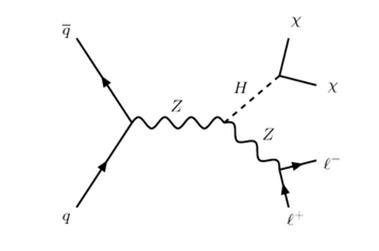
\includegraphics[scale=0.7]{HZ.png}
		\caption{Feynman diagram showing the associated production of a Higgs boson with a Z boson. The Higgs boson decays to two invisible DM particles and the Z boson decays leptonically, resulting in the $ll+ E_T^{miss}$ signature.}
		\label{HZ}
	\end{center}
\end{figure}
The main background processes for the $ll+E_T^{miss}$ final state are $ZZ\rightarrow ll\nu\nu$, $WZ\rightarrow lll\nu$,$WW\rightarrow l\nu l\nu$, $Z+$jets and $W+$jets. The dominant source of background is the $ZZ \rightarrow ll\nu\nu$ process, contributing $\approx 60 \%$ of the background. Figure \ref{fig:ZZdiag} shows the production modes of $ZZ$ from $q\bar{q}$ and $gg$ scattering.\\
A precise estimate of this process, along with the uncertainty associated with it, is crucial. In current analyses, this is determined using simulation, with an uncertainty of $\approx 10\%$ \cite{ZH_ATLAS}.
\begin{figure}[H]
	\begin{center}
		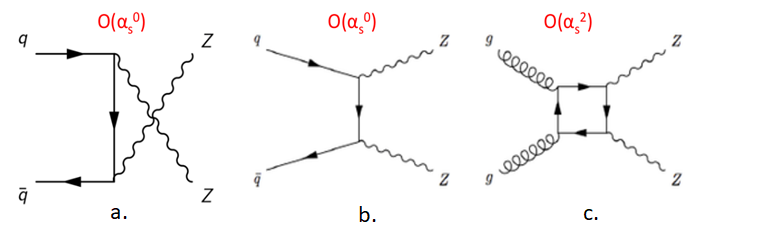
\includegraphics[scale=0.5]{ZZ.png}
		\captionsetup{justification=centering}
		\caption{Feynman Diagram showing $ZZ$ Production \\ a. $q\bar{q}\rightarrow ZZ$, u-channel \hspace{1 cm} b. $q\bar{q}\rightarrow ZZ$, t-channel \hspace{1cm} c. $gg\rightarrow ZZ$}
		\label{fig:ZZdiag}
	\end{center}
\end{figure}

One method of estimating this contribution is to look at $ZZ\rightarrow llll$, which has a branching fraction of $\approx 0.46 \%$. This is due to the low branching fraction of $Z\rightarrow ll$ \footnote{The branching fraction of $Z$ to any one flavor of lepton is $\approx 3.4\%$, and to neutrinos is $\approx 20\%$.}, and is thus statistically limited. Only electrons and muons are considered here as the leptonic decay products of the $Z$ bosons. In contrast, the branching fraction of \ZZ is 2.7\%, about 6 times higher than $ZZ\rightarrow llll$.

As in earlier analysis that used $\gamma+$jets to calibrate $Z+$jets background \cite{gammajet}, in high $Z$ boson $p_T$ regions, the \Zgam process should be kinematically similar to \ZZ, as the mass of the $Z$ boson becomes negligible as compared to the high $Z$ boson $p_T$. Figures \ref{fig:ZZdiag} and \ref{fig:Zgdiag} show the leading order Feynman diagrams for the production of $ZZ$ and $Z+\gamma$ respectively. The diagrams for $q\bar{q}$ and $gg$ (a. b. and c.) are similar. Diagram \ref{fig:Zgdiag}d. corresponds to the production of a single $Z$ boson, with the photon radiated from a final state lepton.\\
In addition to having a higher $BR*\sigma$ as compared to \ZZ (2.7\% for \ZZ vs 6.8\% for \Zgam), the \Zgam signal is also very pure. Thus, it should be possible to use \Zgam data to estimate \ZZ contribution to the background, and obtain a more accurate prediction.
\begin{figure}[h]
	\begin{center}
		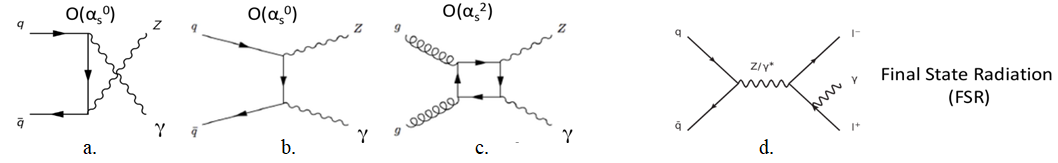
\includegraphics[width=\linewidth]{Zg.png}
		\captionsetup{justification=centering}
		\caption{Feynman Diagram showing $Z+\gamma$ Production} 
		\begin{tabular}{l}
		$q\bar{q}\rightarrow Z+\gamma$,u-channel\\ 
		b. $q\bar{q}\rightarrow Z+\gamma$,t-channel\\ 
		c. $gg\rightarrow Z+\gamma$ \\ 
		d. Final State Radiation (FSR)
		\end{tabular}
		\label{fig:Zgdiag}
	\end{center}
\end{figure}
\section{Approach}
To estimate the background, a transfer factor $R(p_T)$, it is defined to be the ratio of the cross sections of \ZZ to \Zgam as a function of $p_T$, is introduced.
\begin{equation}
	R(p_{T}) = \frac{\sigma_{ZZ}(p_{T})}{\sigma_{Z\gamma}(p_T)}
\end{equation}
With the two processes being kinematically similar at high $p_T$, $R$ depends on the coupling of the $Z$ and $\gamma$ to quarks. It would be expected to reach a constant value at high $p_T$ that can be determined theoretically. In the following paragraph, an attempt is made to obtain a simple approximate calculation of $R$ from the contribution of $qq$ process.

The photon - quark and $Z$ boson - quark couplings in the Standard Model are given by,
\begin{equation}
	-ieQ_q\gamma^{\mu} \hspace{1 cm} \text{and} \hspace{1 cm}\frac{-ie}{2 \sin\theta_W \cos\theta_W}\gamma^{\mu}(v_q - a_q\gamma_5)
\end{equation}
respectively, where $Q_q,v_q$ and $a_q$ are respectively the electric, vector and axial neutral weak couplings of the quarks, and $\theta_W$ is the weak mixing angle. There is a contribution due to the $Z$ mass which appears in the internal propagators and phase space integration. This contribution becomes less important in the $p_T(\gamma)\gg M_Z$ region.

Thus, the leading order contributions from $q\bar{q}\rightarrow ZZ$ and $q\bar{q}\rightarrow Z\gamma$ are shown in Equation \ref{eq:theory_R}.
\begin{equation}
\begin{split}
	\sigma(q\bar{q}\rightarrow ZZ) &\propto \frac{1}{2}\frac{e^2\{(v_q^2 + a_q^2)^2 + 4v_q^2a_q^2\} }{16\sin^4\theta_W\cos^4\theta_W}\\[1.5ex]
	\sigma(q\bar{q}\rightarrow Z\gamma) &\propto \frac{e^2Q_q^2(v^2_q + a^2_q)}{4\sin^2\theta_W\cos\theta_W}
\end{split}
\label{eq:theory_R}
\end{equation}
The $u$ and $d$ quarks present in a $pp$ collision have different coupling strengths to the $Z$ boson as stated in Ref\cite{Z_coupling}, their relative contributions are accounted for using Equation \ref{eq:u_d_contrib}
\begin{equation}
R = \frac{\sigma(u\bar{u}\rightarrow ZZ)\langle u\rangle + \sigma(d\bar{d}\rightarrow ZZ)\langle d\rangle}{\sigma(u\bar{u}\rightarrow Z\gamma)\langle u\rangle + \sigma(d\bar{d}\rightarrow Z\gamma)\langle d\rangle}
\label{eq:u_d_contrib}
\end{equation}
Using the vector and axial couplings of the $Z$ boson to $u$ and $d$ quarks, assuming $\langle d \rangle/\langle u\rangle = 0.5$ and setting $\sin^2\theta_W = 0.2315$, $R\approx 1.28$ for the dominant $qq$ interaction.

\subsection*{Theoretical determination of MCFM cross sections}
A Monte Carlo program, MCFM v8.0 \cite{MCFM} at NLO is used to generate cross sections of \ZZ and \Zgam processes, with a selection of generator level cuts. The samples are generated with cuts on $E_T^{miss} = p_T(Z\to \nu\nu)$ for the $ZZ$ process and $E_T^{miss} = p_T(\gamma)$ for the $Z+\gamma$ process. A ratio of these cross sections is taken to obtain the $R$ distribution as a function of $p_T$. The uncertainty on $R$ is calculated by varying several parameters at the generator level, such as the renormalization and factorization scales, the PDF sets used, photon fragmentation, etc. Effects of applying lepton cuts on the cross sections as well as on the ratio are studied. The contributions of the $q \bar{q}$ and $gg$ processes are estimated separately.

MCFM does not generate $Z\rightarrow ll$ but $Z\rightarrow ee$. As electrons and muons have similar properties with the exception of mass, simply the branching fraction of $Z\rightarrow ee$ must be accounted for to obtain the inclusive value of $R$.
\begin{equation}\label{eq:R_inc}
	R_{inc} = R * \frac{BR(Z\rightarrow ee)}{BR(Z \rightarrow ee)*BR(Z\rightarrow \nu\nu)*2}
\end{equation}

\section{Generator Parameters}
The samples are generated using MCFM v8.0 for the following data points:
\begin{align*}
	\text{For } ZZ \rightarrow ee\nu\nu &: E_T^{miss} > \{50,75,100,125,150,200,250,300,400,500\}\text{ GeV} \\
	\text{For } Z(\rightarrow ee)+\gamma &: p_T(\gamma) > \{50,75,100,125,150,200,250,300,400,500\}\text{ GeV}
\end{align*}
Table \ref{table:default} lists the generator level settings used for the $ZZ$ and $Z+\gamma$ processes. All lepton cuts are consistent with the ones used in the ATLAS Z+$E_T^{miss}$ analysis.
\begin{table}[H]
\begin{center}
	\begin{tabular}{|c|c|c|}
	\hline
	\textbf{Cuts} &$ZZ \rightarrow ee\nu\nu$ & $Z(\rightarrow ee)+\gamma$\\
	\hline
	Process ID & 87 & 300\\
	$M_{ee}$ & $81 < M_{ee} < 101$ GeV & $81 < M_{ee} < 101$ GeV\\
	$M_{\nu\nu}$ & $81 < M_{\nu\nu} < 101$ GeV& -\\
	Order & NLO & NLO\\
	PDF set & CT14 & CT14\\
	$p_T^{\text{lead}}(e)$ & $> 30$ GeV & $> 30$ GeV\\
	$|\eta^{lead}(e)|$ & $< 2.5$ & $< 2.5$\\
	$p_T^{\text{sublead}}(e)$ & $> 20$ GeV & $> 20$ GeV\\
	$|\eta^{sublead}(e)|$ & $< 2.5$ & $< 2.5$\\
	$\Delta R(\gamma,e)$ & - & 0.7\\
	Renormalization scale & $91.187$ GeV $(M_{Z})$& $91.187$ GeV $(M_{Z})$\\
	Factorization scale & $91.187$ GeV $(M_{Z})$& $91.187$ GeV $(M_{Z})$\\
	\hline
	\end{tabular}
	\caption{Settings in input.DAT for MCFM}
	\label{table:default}
	\end{center}
\end{table}
The constraint on $M_{ee}$ in the case of $Z+\gamma$ suppresses the FSR process by ensuring that the lepton pair are from a $Z$ decay only.
\section{Results}
Using the settings listed in Table \ref{table:default}, the cross sections shown in Figure \ref{xsecs} are obtained. Throughout this analysis, this sample is the reference.
\begin{figure}[H]
\centering
	\begin{subfigure}{0.49\textwidth}
		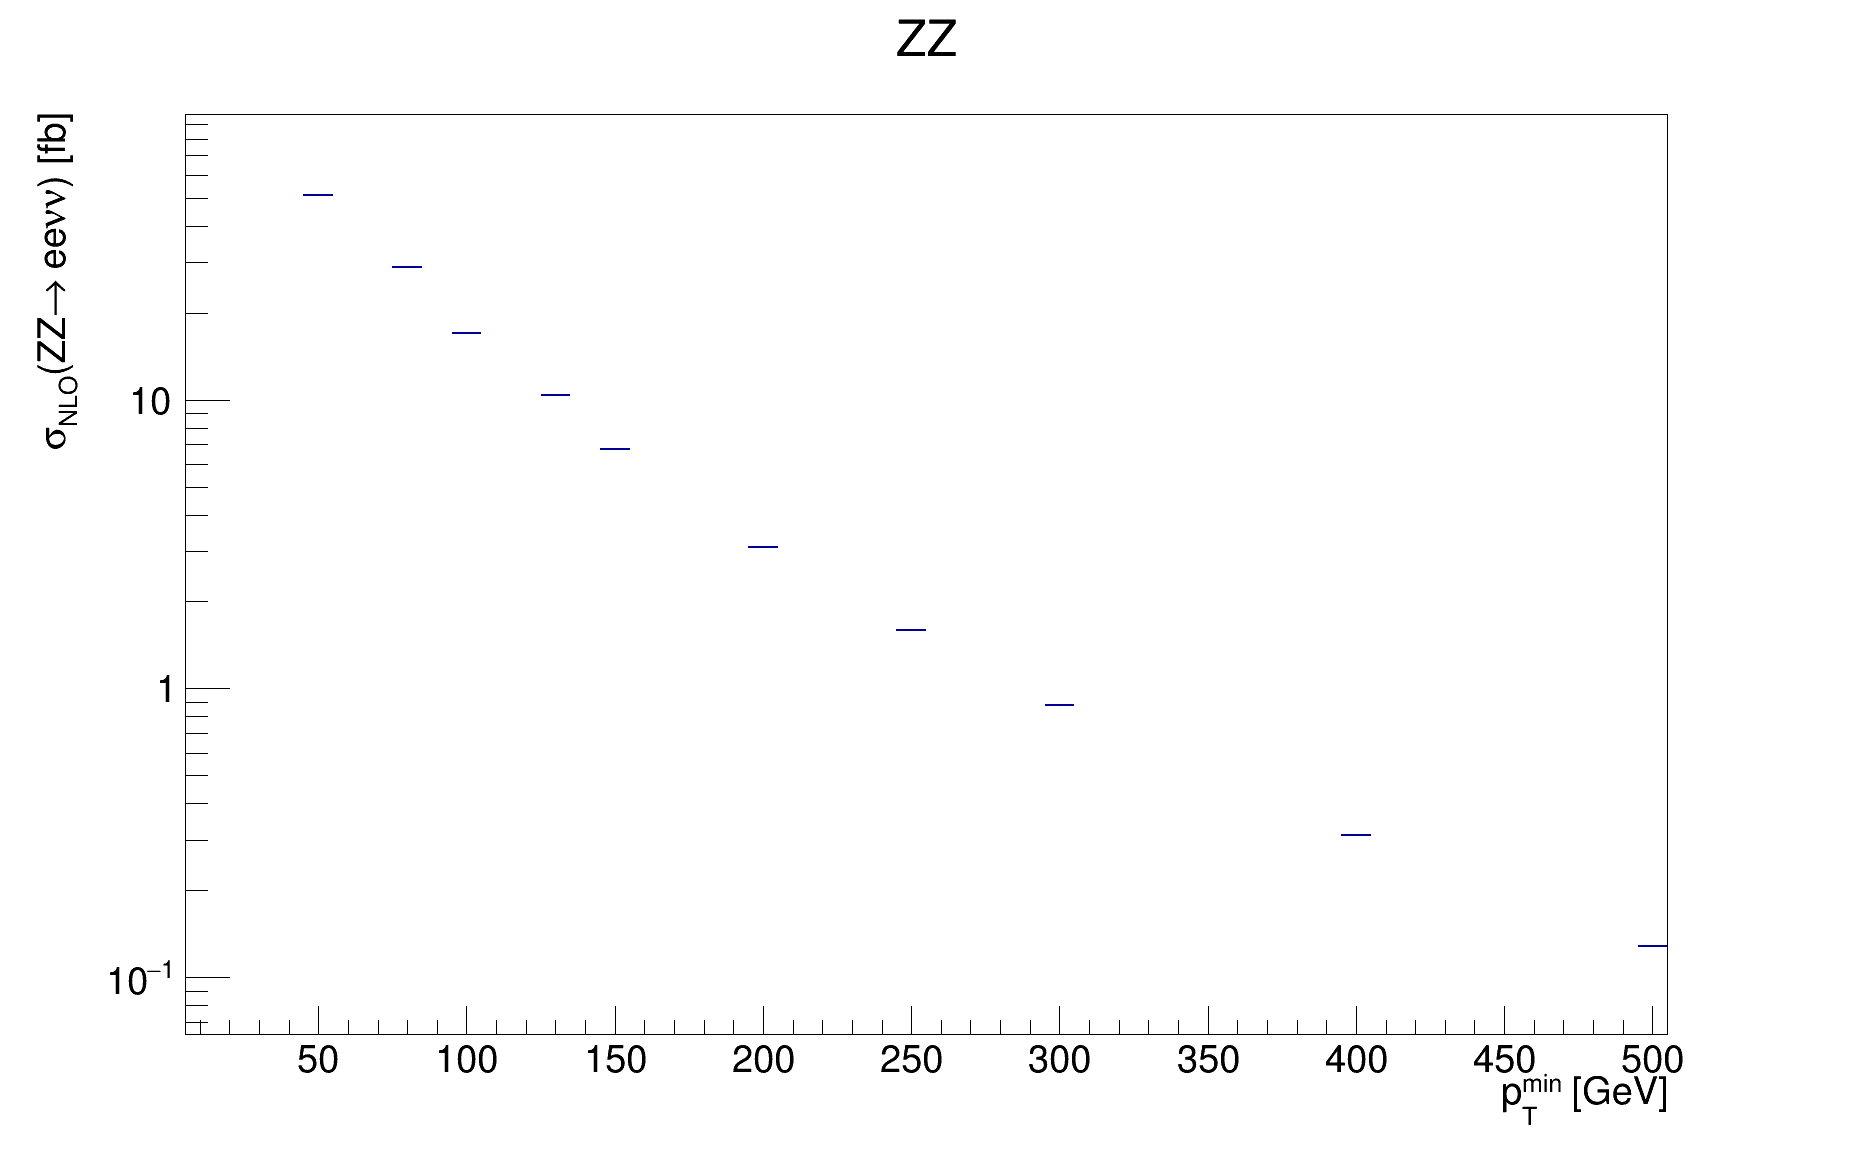
\includegraphics[width=\linewidth]{ZZ_xsec.png}
		\caption{$ZZ\rightarrow ee\nu\nu$ cross section}
		\label{subfig:ZeeZvv}
	\end{subfigure}	
	\begin{subfigure}{0.49\textwidth}
		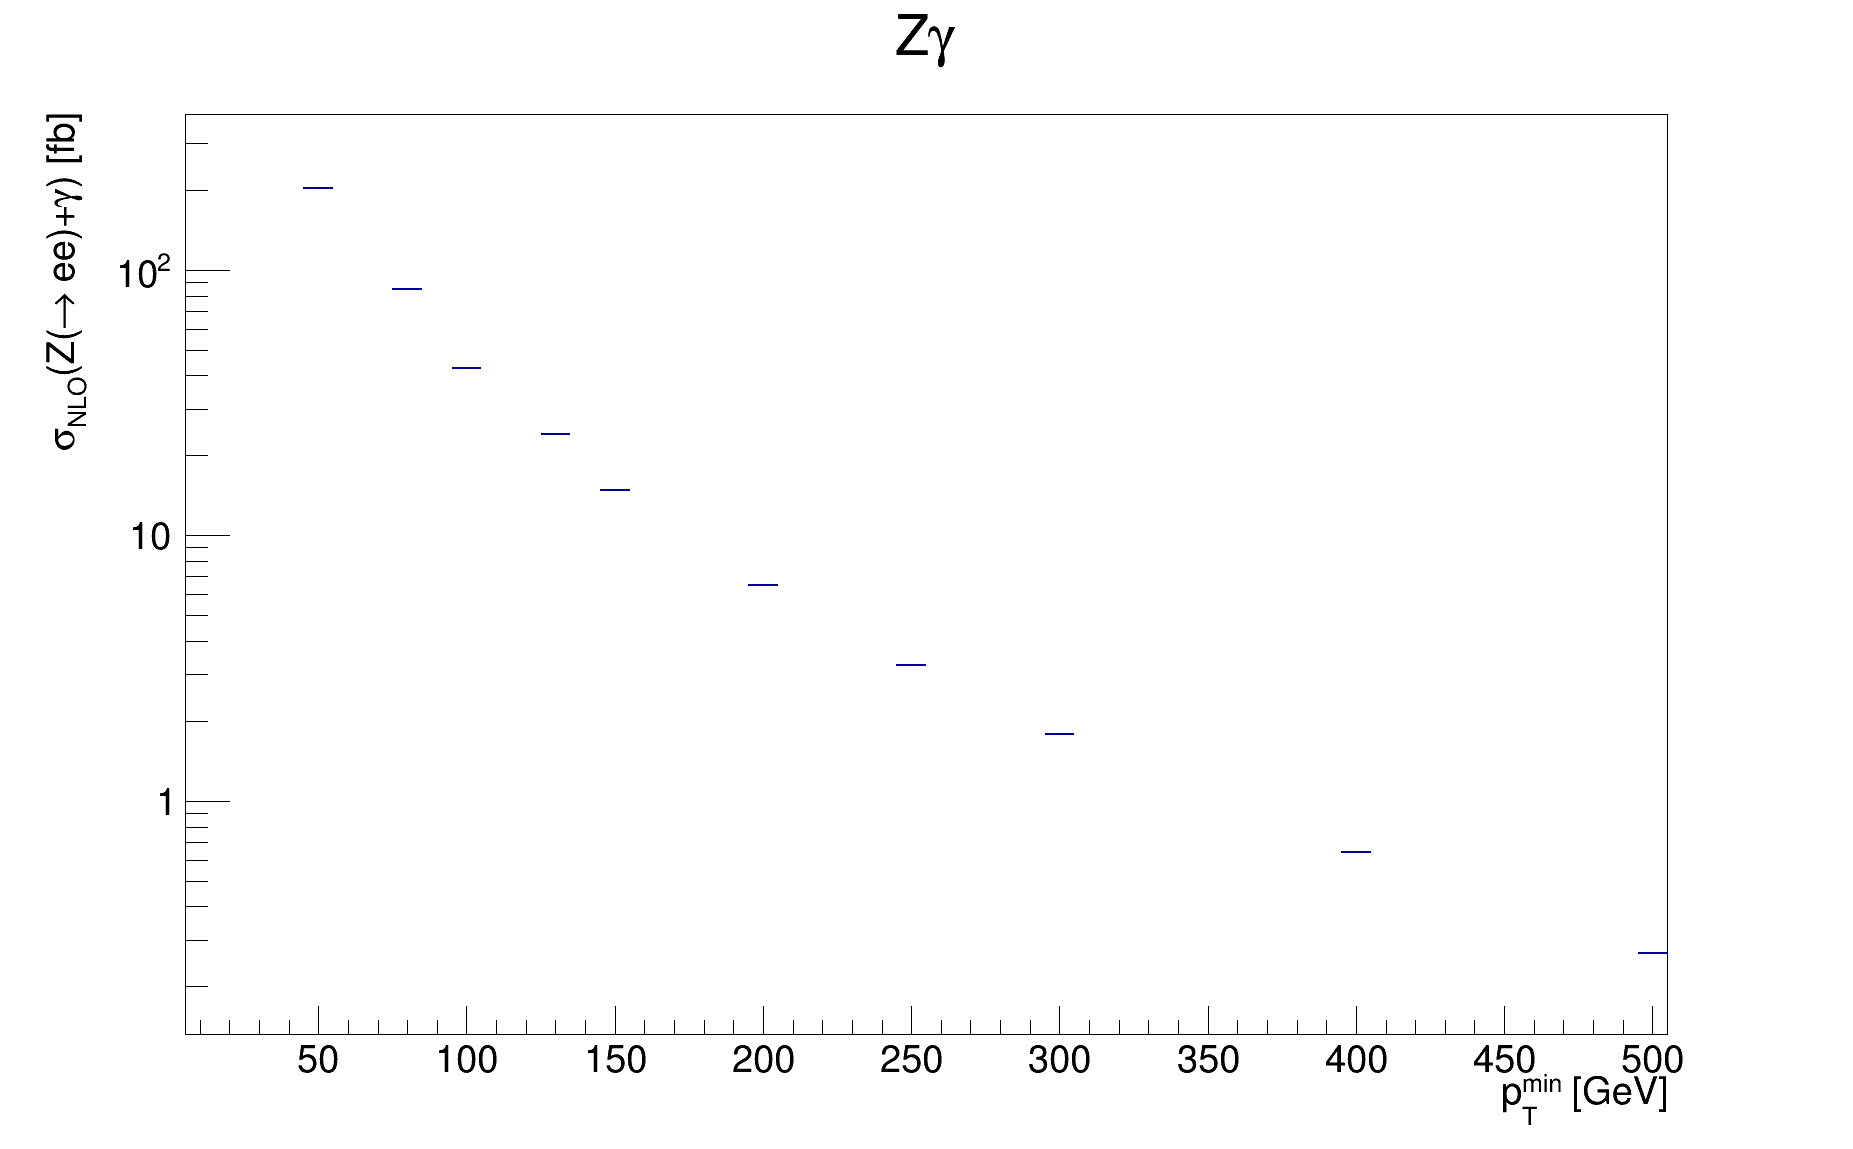
\includegraphics[width=\linewidth]{Zg_xsec.png}
		\caption{$Z(\rightarrow ee)+\gamma$ cross section}
		\label{subfig:Zeeg}	
	\end{subfigure}
	\caption{Cross sections of $ZZ$ and $Z+\gamma$ processes with the cuts as in Table 1. The vertical axis is in $\log_{10}$ scale. The leptonically decaying $Z$ boson decays to an $e^+e^-$ pair. There is no flavor constraint on the neutrinos.}
	\label{xsecs}
\end{figure}
\begin{figure}[H]
	\centering
	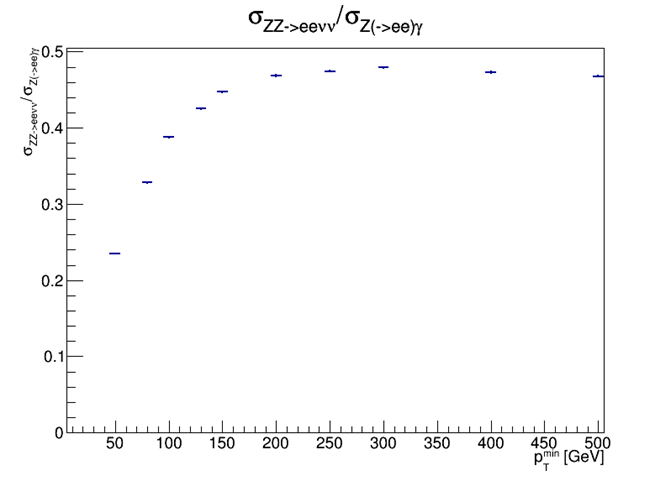
\includegraphics[scale=0.7]{Ratio_default.png}
	\caption{The transfer factor $R$ as a function of $p_T$, taken as a ratio of plots \ref{subfig:ZeeZvv} and \ref{subfig:Zeeg}. The leptonically decaying $Z$ boson decays to an $e^+e^-$ pair.}
	\label{fig:Rcurve}
\end{figure}
The ratio $R = \sigma(ZZ\rightarrow ee\nu\nu)/\sigma(Z\gamma\rightarrow ee\gamma)$ is shown in Figure \ref{fig:Rcurve}. The $R$ value is observed to increase from $\approx 0.24$ at 50 GeV to $\approx 0.47$ at high $p_T$, where it is constant. When the branching ratio of $Z$ boson decaying selectively to $e^+e^-$, or to $\nu\nu$, is accounted for as shown in Equation \ref{eq:R_inc}, the resulting ratio $R(p_T)$ is shown in Figure \ref{fig:RcurveBR}, which shows the ratio of $\sigma(ZZ)$ to $\sigma(Z\gamma)$, i.e. if the $Z$ bosons do not decay further. The value of $R$ is observed to increase from $\approx 0.61$ at 50 GeV to $\approx 1.2$ at high $p_T$, in reasonable agreement with the simple approximate calculation presented in Section 2 of $R \approx 1.28$.
\begin{figure}[H]
	\centering
	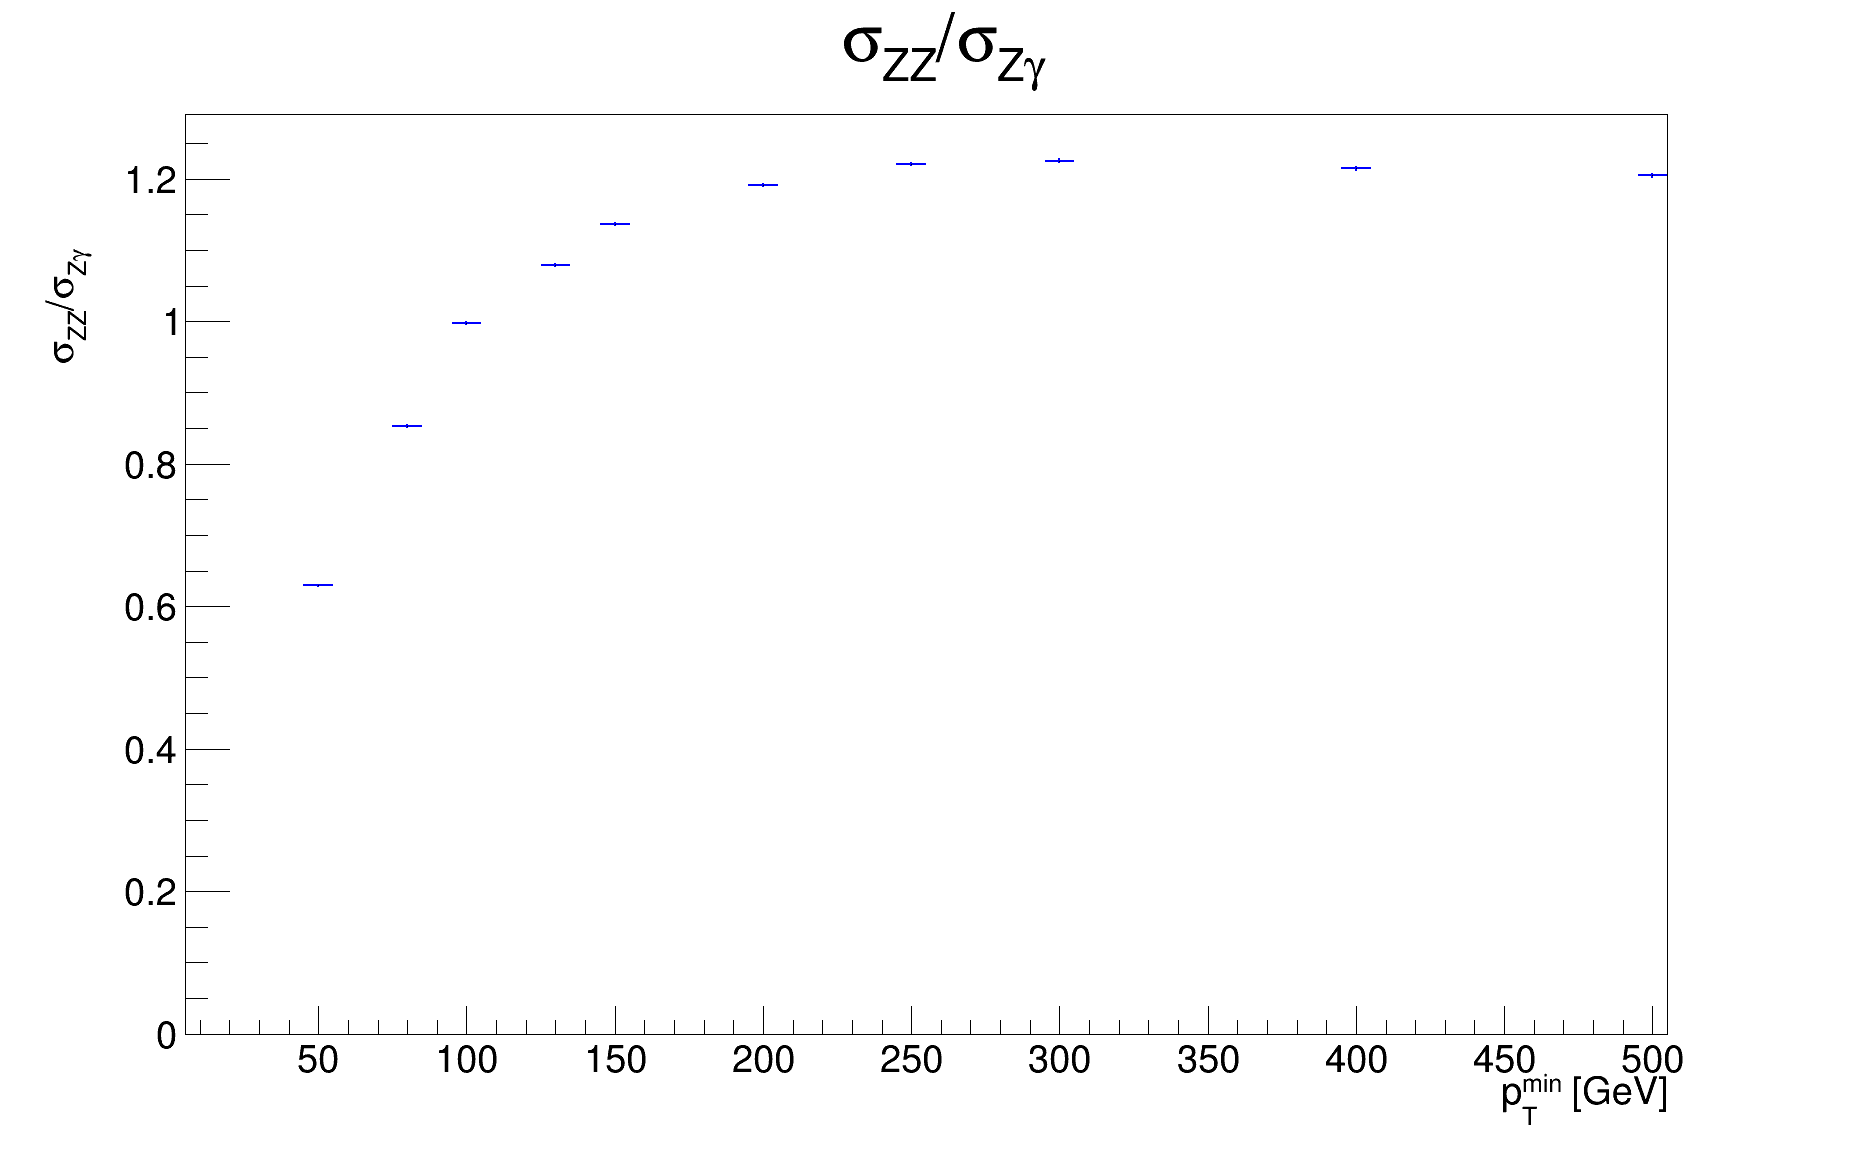
\includegraphics[width = 0.8\textwidth]{Ratio_with_BR.png}
	\caption{The transfer factor $R$ as a function of $p_T$, adjusted for the $Z\rightarrow ee$ and $Z\rightarrow \nu\nu$ branching ratios. This shows the $R=\sigma(ZZ)/\sigma(Z\gamma)$, where the $Z$ bosons do not decay.}
	\label{fig:RcurveBR}
\end{figure}

Gluon-gluon processes contribute to 8.6\% of the total cross section for the $ZZ$ process and 2.5\% of the $Z+\gamma$ process. Figure \ref{fig:R_gg_qq} shows the transfer factor $R$ obtained from the $gg$ process, as well as $R$ from the $q\bar{q}$ and $qg$ processes.
\begin{figure}[H]
\centering
	\begin{subfigure}{0.49\textwidth}
		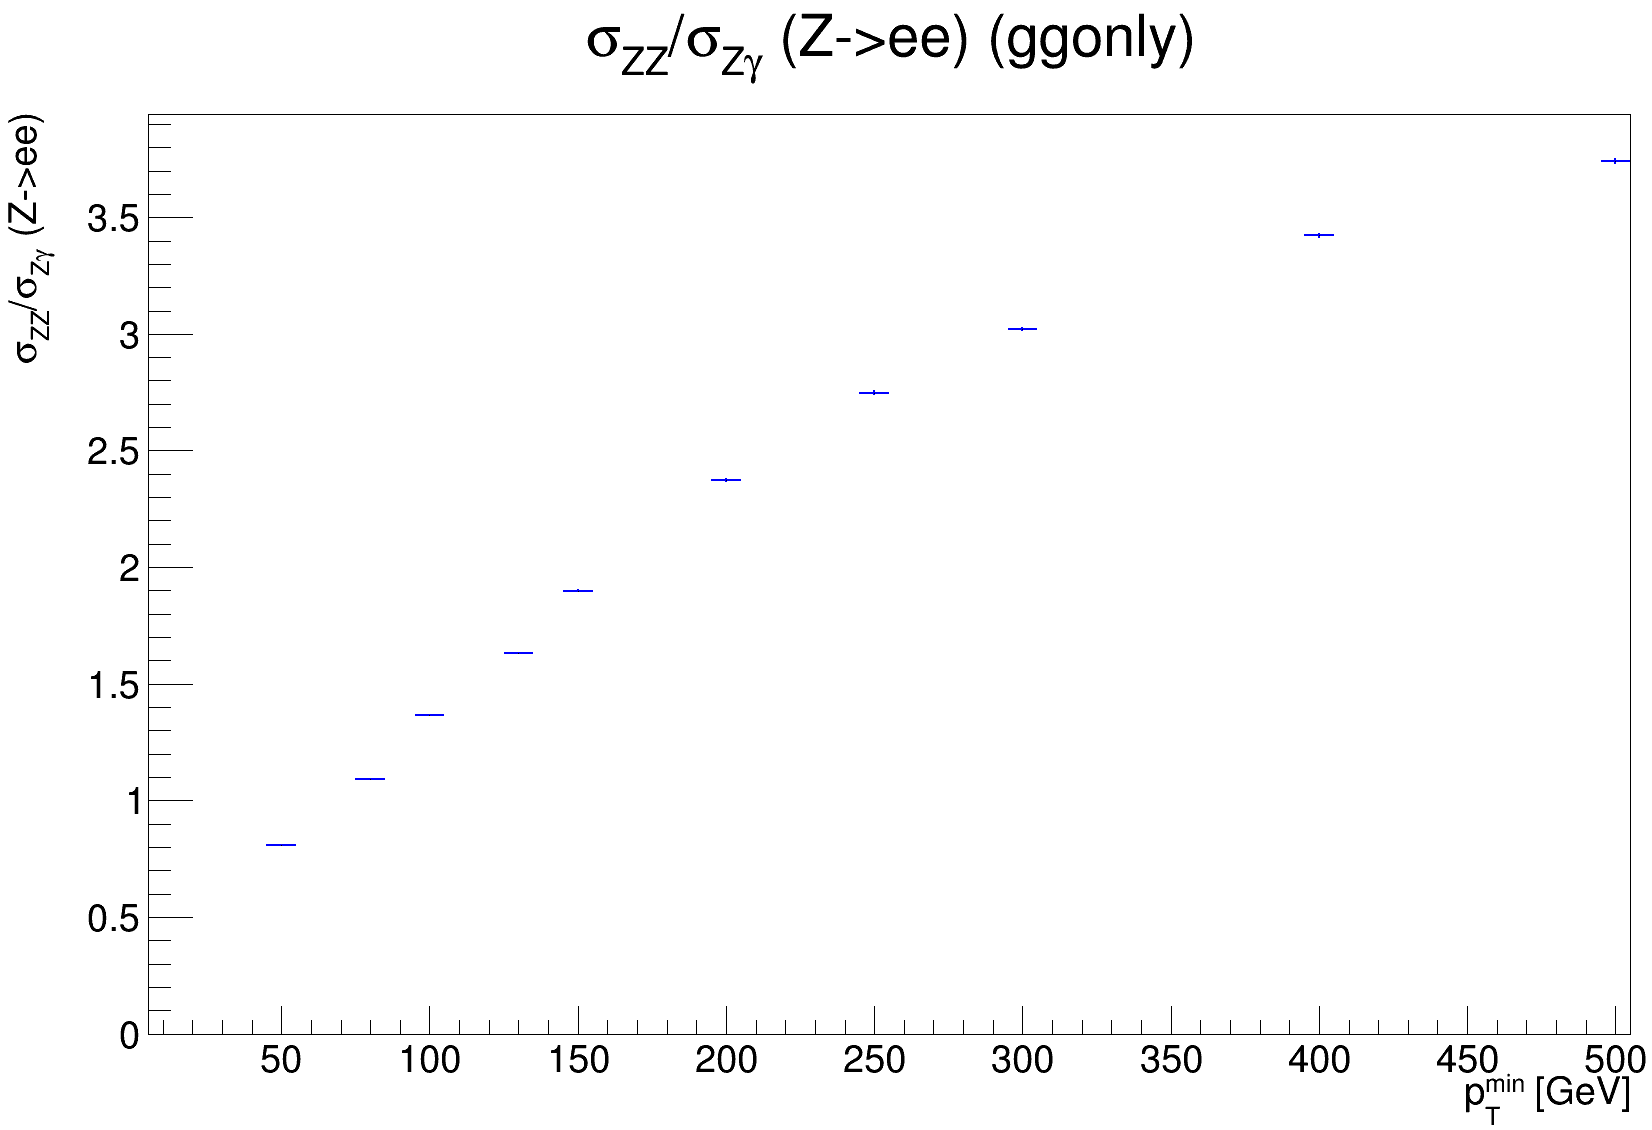
\includegraphics[width=\linewidth]{R_ggonly.png}
		\caption{}
		\label{subfig:R_gg}
	\end{subfigure}
	\begin{subfigure}{0.49\textwidth}
		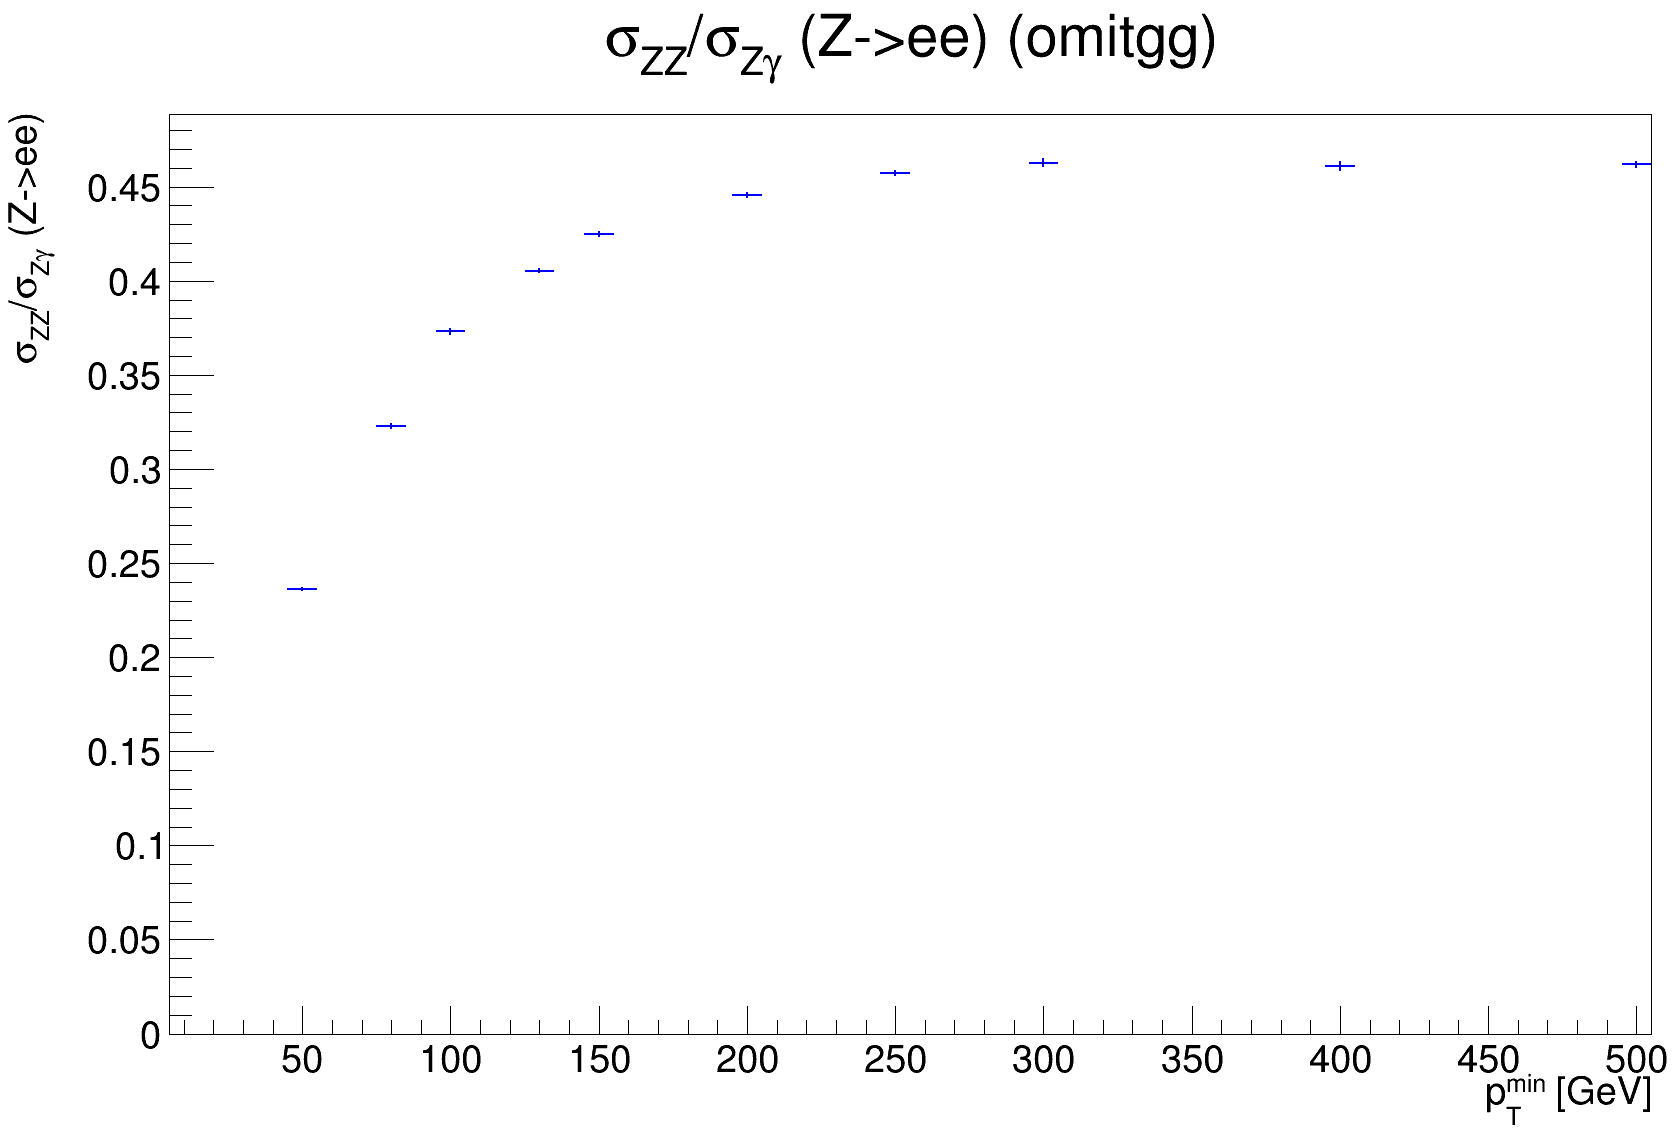
\includegraphics[width=\linewidth]{R_omitgg.png}
		\caption{}
		\label{subfig:R_qq}
	\end{subfigure}	
\caption{$R(p_T)$ from the contributing $gg$ processes (a), and $qg$ and $q\bar{q}$ processes together (b). The $Z$ bosons decay further to $e^+e^-$ for the leptonic $Z$ boson, or $\nu\nu$ for the invisibly decaying $Z$ boson.}
\label{fig:R_gg_qq}
\end{figure}
The $R_{gg}$ distribution is observed to approach an asymptotic value at a much higher $p_T = 1.5$ TeV. The shape and scale of the $R_{gg}$ distribution (Figure \ref{subfig:R_gg}) remain to be understood, as they differ from Figure \ref{fig:Rcurve}.

\subsection{Effect of Lepton Cuts}
To check the effects of lepton cuts on the ratio, samples with the same parameters as those in Table \ref{table:default} are generated. However, we relax the cuts on leptons. Both the leading and subleading lepton should have $p_T > 5$ GeV, and $\eta <$ 10. In the lower $p_T$ regions, the cross section falls by nearly half in both processes. The ratio is affected by up to 15\% as seen in Figure \ref{fig:lepcut}, and therefore for all following studies the lepton cuts are applied as they emulate the experimental cuts needed in the analysis.
\begin{figure}[H]
\centering
	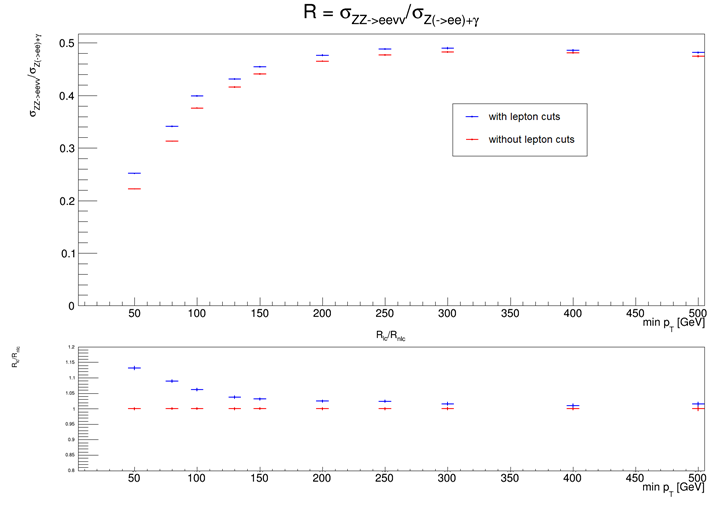
\includegraphics[width = 0.8\linewidth]{lep_cuts.png}
	\caption{Comparison of reference the $R$ distribution to the $R$ distribution without lepton cuts}
	\label{fig:lepcut}
\end{figure}
\subsection{Uncertainty from Scale Variation}
In higher order QCD calculations, perturbative corrections may be added to the vertices or propagators in a Feynman diagram. Physically, these corrections occur at very small time scales. These loop integrals that correspond to these corrections diverge.\\
The higher the order, the more difficult the calculation is. It is possible to introduce an arbitrary cut-off scale $\mu$ such that up to a given order, the effect of these corrections can be absorbed into the strong coupling constant $\alpha_s(\mu)$.\\
Two kinds of divergences are encountered: infrared divergences, and ultraviolet divergences. Infrared divergences occur for an on-shell internal propagator, and ultraviolet divergences are logarithmic divergences that occur as the integration variable approaches $\infty$. They correspond to physics at long and short distances\footnote{Long distances are those where soft interactions take place, away from the hard parton-parton interaction. Short distances are those where the hard parton parton interactions occur.}, respectively. The infrared divergences are addressed by the inclusion of the factorization scale $\mu_F$, while the ultraviolet divergences are addressed by the inclusion of the renormalization scale $\mu_R$. These parameters are arbitrary, and are set by hand. These are then varied between $\frac{1}{2}\mu < \mu < \ 2\mu$ to obtain an indication of the dependence of the matrix element on the scales, and thus, the uncertainty around the chosen scale. 

In this analysis, the central value for these parameters is chosen to be $M_Z = 91.187$ GeV, and the results are shown in Figure \ref{fig:scalecompare}.
\begin{figure}[H]
\centering
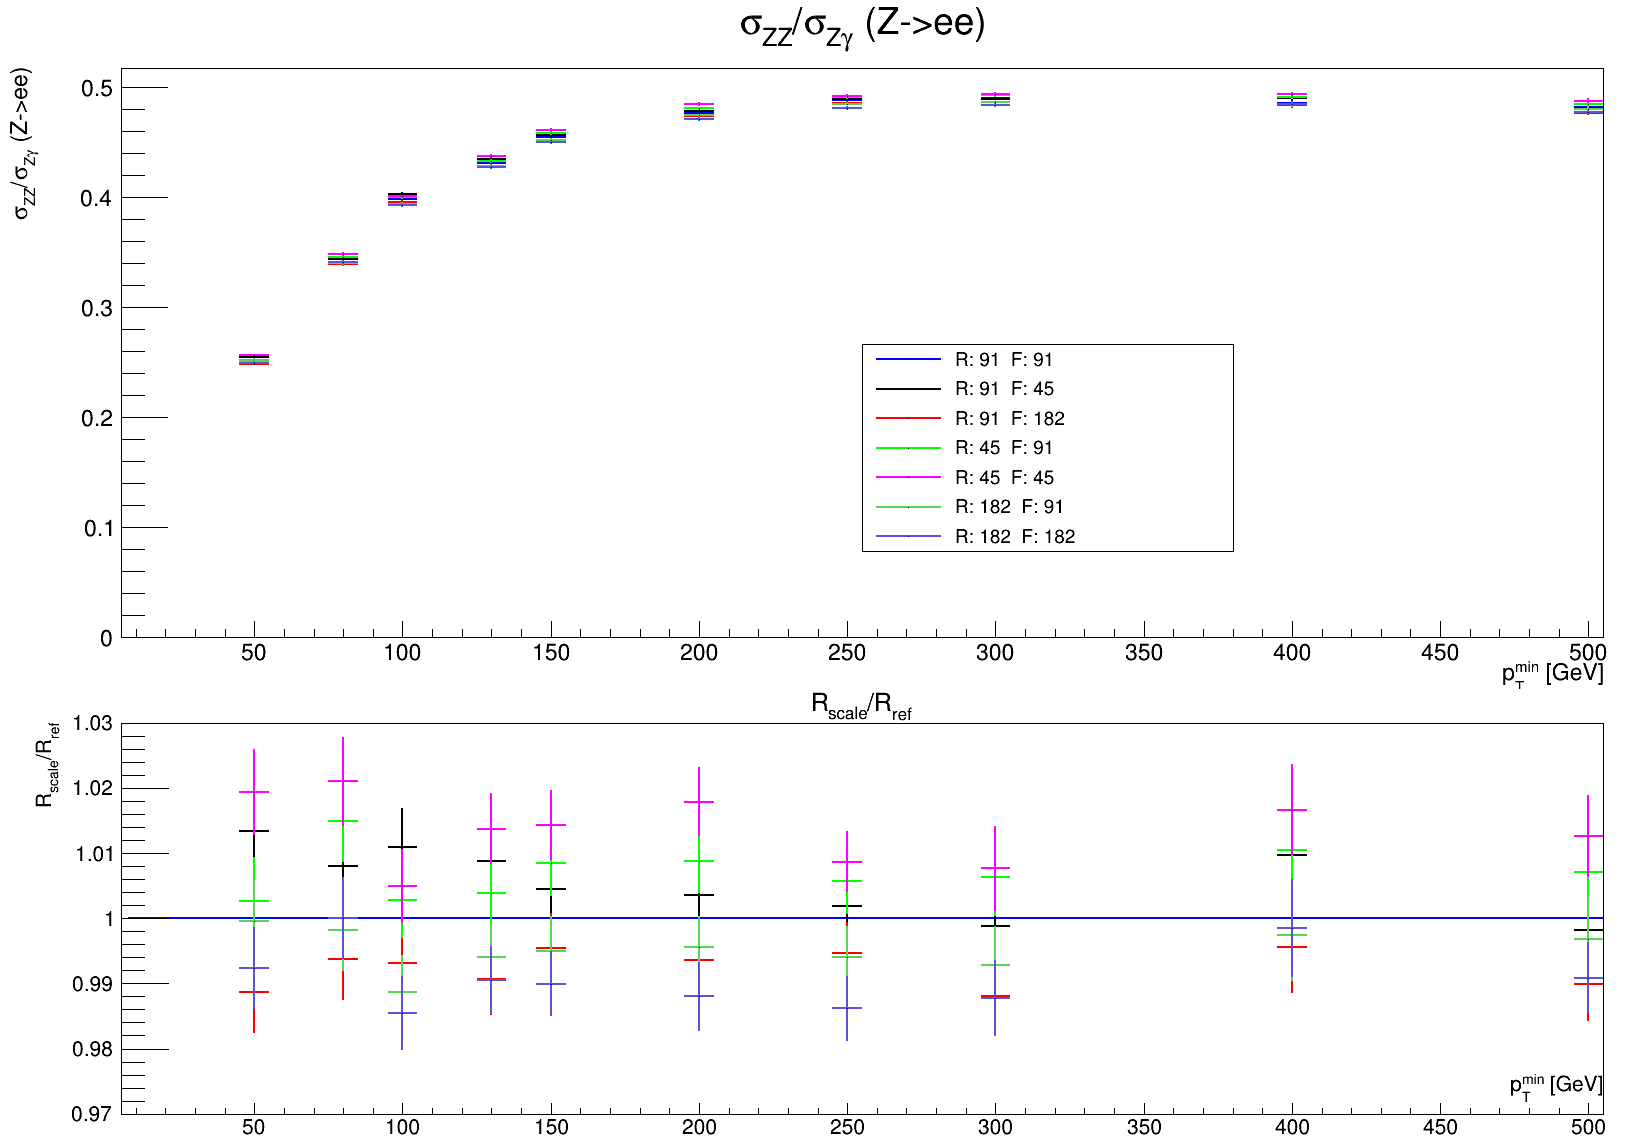
\includegraphics[width=0.8\linewidth]{scale/nlo_scale_overlay.png}
\caption{The ratio $R(p_T)$ for various choices for $\mu_R$ (R) and $\mu_F$ (F). The bottom panel shows the relative - with respect to the reference (R: 91, F: 91) for each scale. The uncertainties are statistical}
\label{fig:scalecompare}
\end{figure}
The uncertainty due to the variation of scales around $R = 0.398$ is $\pm \approx 2\%$ for all $p_T$.\\
The contributions from the $gg$ subprocess separately from the $q\bar{q}$ and $qg$ subprocesses are shown in Figure \ref{fig:gg_scale}.
\begin{figure}[H]
\centering
	\begin{subfigure}{0.49\textwidth}
		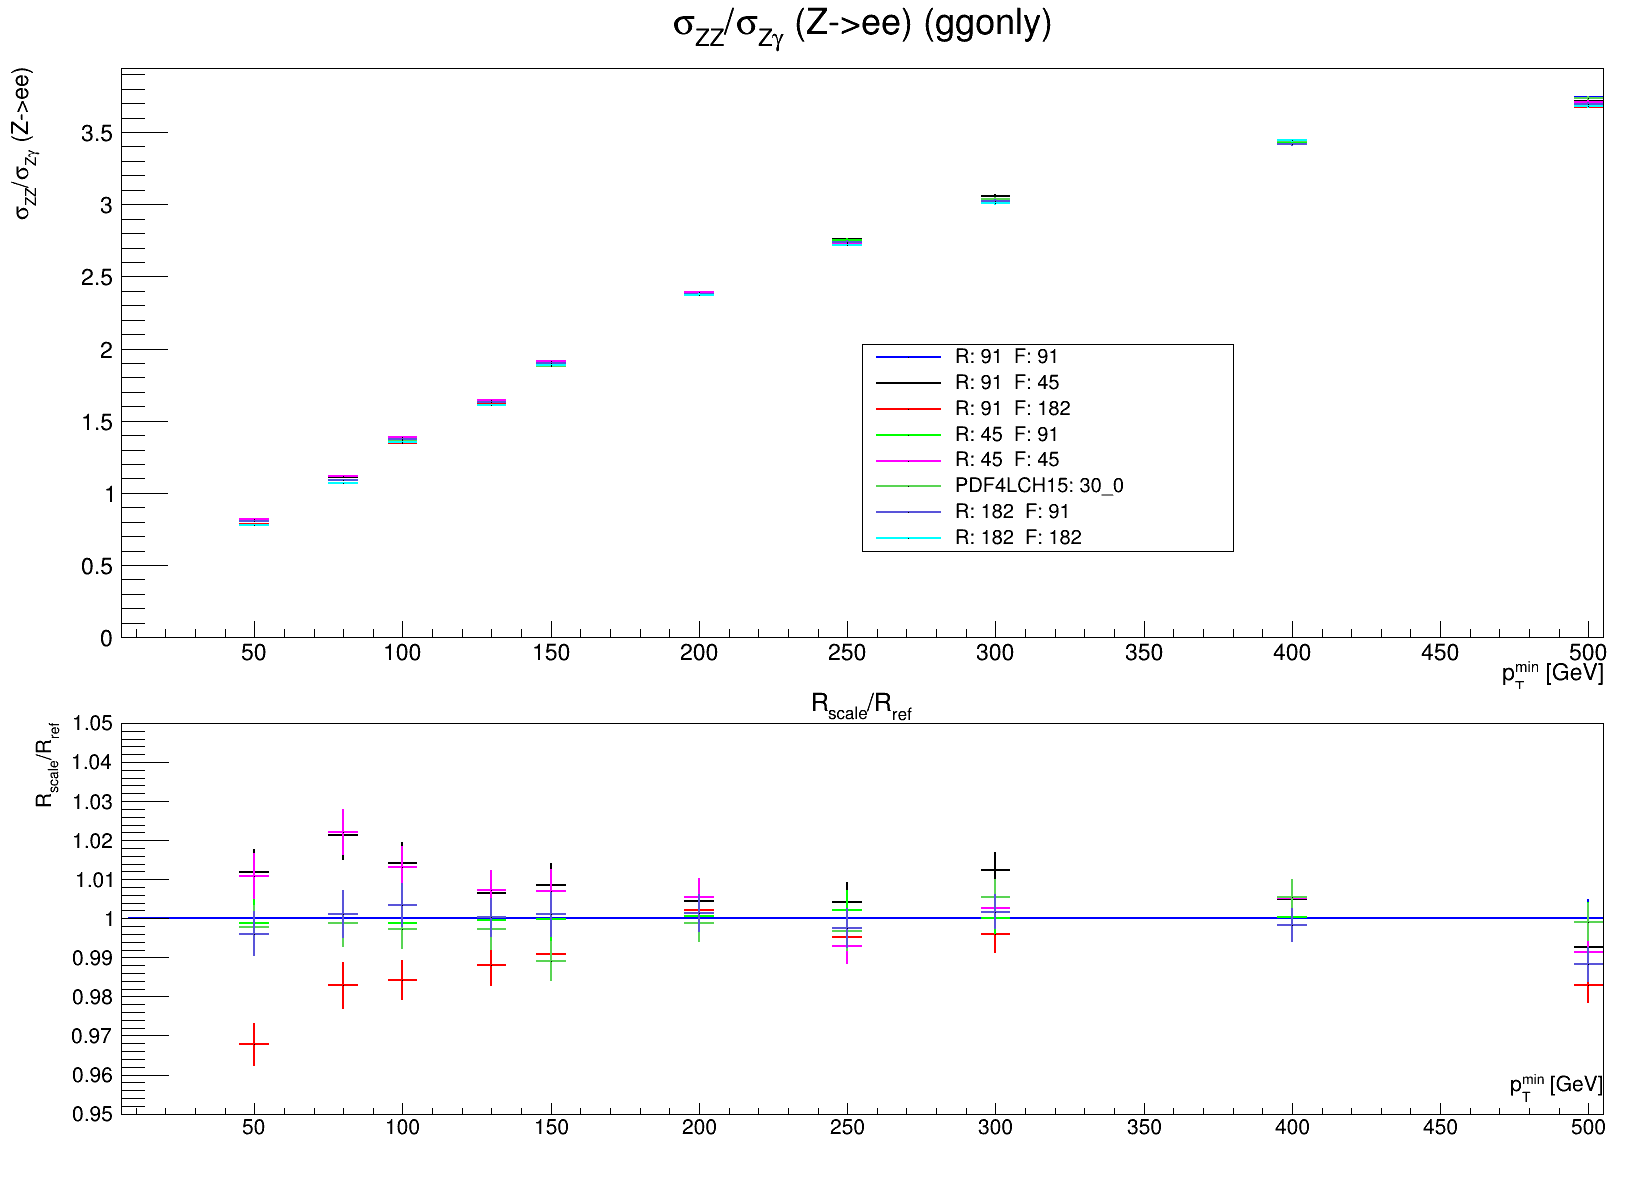
\includegraphics[width=\linewidth]{scale/ggonly_nlo_scale_overlay.png}
		\caption{$R_{gg}$ from $gg$ subprocess only}
	\end{subfigure}
	\begin{subfigure}{0.49\textwidth}
		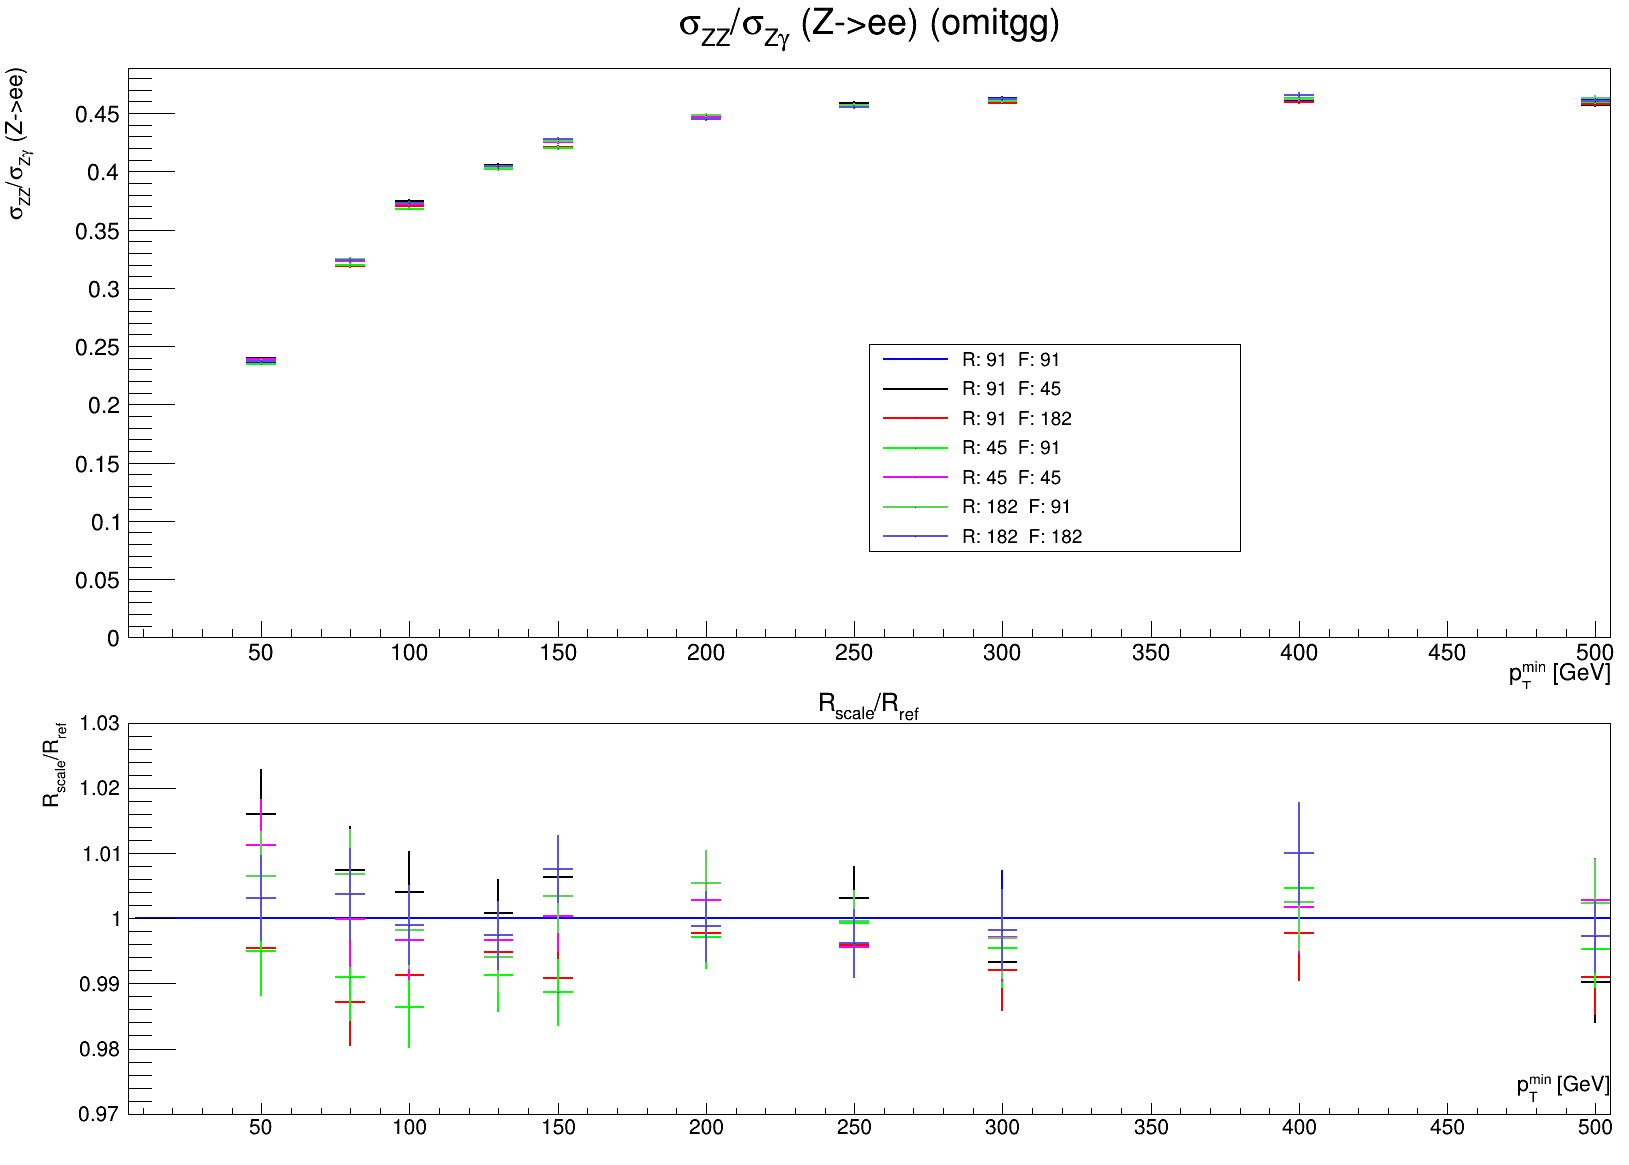
\includegraphics[width=\linewidth]{scale/omitgg_nlo_scale_overlay.png}
		\caption{$R_{q\bar{q}/qg}$ from $q\bar{q}$ and $qg$ subprocesses}
	\end{subfigure}	
\caption{The ratio $R(p_T)$ for various choices for $\mu_R$ (R) and $\mu_F$ (F) for the $gg$ and $qg+q\bar{q}$ subprocesses separately. The bottom panel shows the relative difference with respect to the reference (R: 91, F: 91) for each scale. The uncertainties are statistical.}
\label{fig:gg_scale}
\end{figure}

Variations of up to 3\% are seen at low pt while at high pt the differences are below 1\% for the plots show in Figures \ref{fig:scalecompare} and \ref{fig:gg_scale}

\subsection{Uncertainty from PDF variation}
Parton Distribution Functions (PDFs) characterize the fraction of proton momentum carried by partons as probability distributions. PDF sets are collections of PDFs that model parton momenta as accurately as possible. The PDF set used for reference is the \texttt{CT14}\cite{CT14} PDF set. The uncertainty on the PDFs is studied by using the 30 variations provided by the \texttt{PDF4LHC15} set\cite{PDF4}, constructed from the combination of \texttt{CT14,MMHT14}\cite{MMHT14} and \texttt{NNPDF3.0}\cite{NNPDF3} PDF sets. These sets are provided by LHAPDF6\cite{LHAPDF}. \texttt{PDF4LHC15} provides a set of variations that include those determined by different groups (MSTW, CTEQ and NNPDF). The set used here is \texttt{PDF4LHC15\_nlo\_30}, consisting of 30 members. While the most accurate uncertainties are given by \texttt{PDF4LHC15\_nlo\_100} set, \texttt{PDF4LHC15\_nlo\_30} is used here for a faster, reasonably accurate estimate of the uncertainties.
\begin{figure}[H]
\centering
	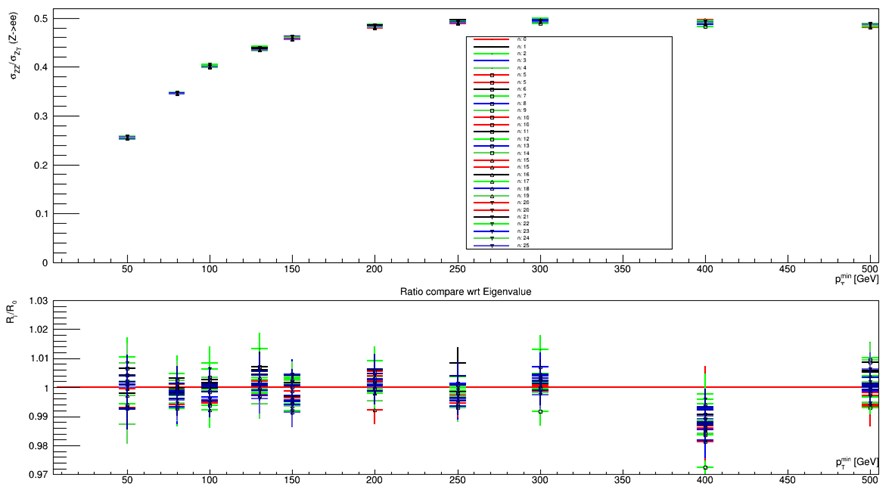
\includegraphics[width = 0.8\linewidth]{PDF4_30_overlay.png}
	\caption{The ratio $R(p_T)$ for each of the 30 PDF sets in \texttt{PDF4LHC15\_nlo\_30}. The bottom plot shows the relative differences of sets 1-30, with respect to set 0 which is taken as the central value.}
	\label{fig:PDF30var}
\end{figure}
\noindent Fig.\ref{fig:PDF30var} shows the comparison of the ratio $R(p_T)$ from the 30 member sets of \texttt{PDF4LHC15\_nlo\_30}. To measure the uncertainty due to these 30 sets, the relation as stated in Equation 20 in Ref \cite{PDF4} is used:
\begin{equation}\label{eq:PDFerr}
	\delta^{PDF}\sigma = \sqrt{\sum^{N_{mem}}_{k=1} (\sigma^{(k)} - \sigma^{(0)})^2}
\end{equation}
where $N_{mem}$ is the number of member sets in the group, in this case, 30. The $R$ distribution obtained from the \texttt{PDF4LHC15\_nlo\_30} set is compared to the reference distributions from \texttt{CT14}, as shown in Figure \ref{pdfcompare}:
\begin{figure}[H]
\centering
	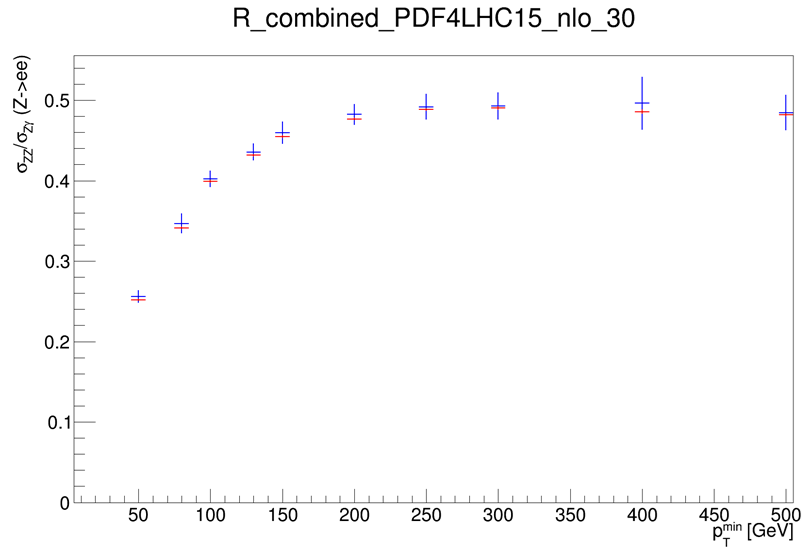
\includegraphics[width = 0.55\linewidth]{PDF4_CT14_comp.png}
	\caption{The ratio $R(p_T)$ calculated using the PDF sets in \texttt{PDF4LHC15\_nlo\_30} with combined uncertainties as given by Equation \ref{eq:PDFerr} (blue), compared to the reference constructed from the PDF set \texttt{CT14} (red).}
	\label{fig:PDF4_def_compare}
	\label{pdfcompare}
\end{figure}
\noindent Figure \ref{fig:PDF4_def_compare} shows a comparison between the central value of the sets in \texttt{PDF4LHC15\_nlo\_30} with the combined uncertainties, and the reference PDF set \texttt{CT14}. The combined uncertainty around $R \approx 0.40$ is $\pm 2.55\%$ at 100 GeV. The $R$ distributions drawn from the two PDF sets agree to within the uncertainty bounds.

%The effect of the PDF uncertainties on $gg$ process are studied separately, as illustrated in Figure \ref{pdfcompare_gg}.
%\begin{figure}[H]
%\centering
%	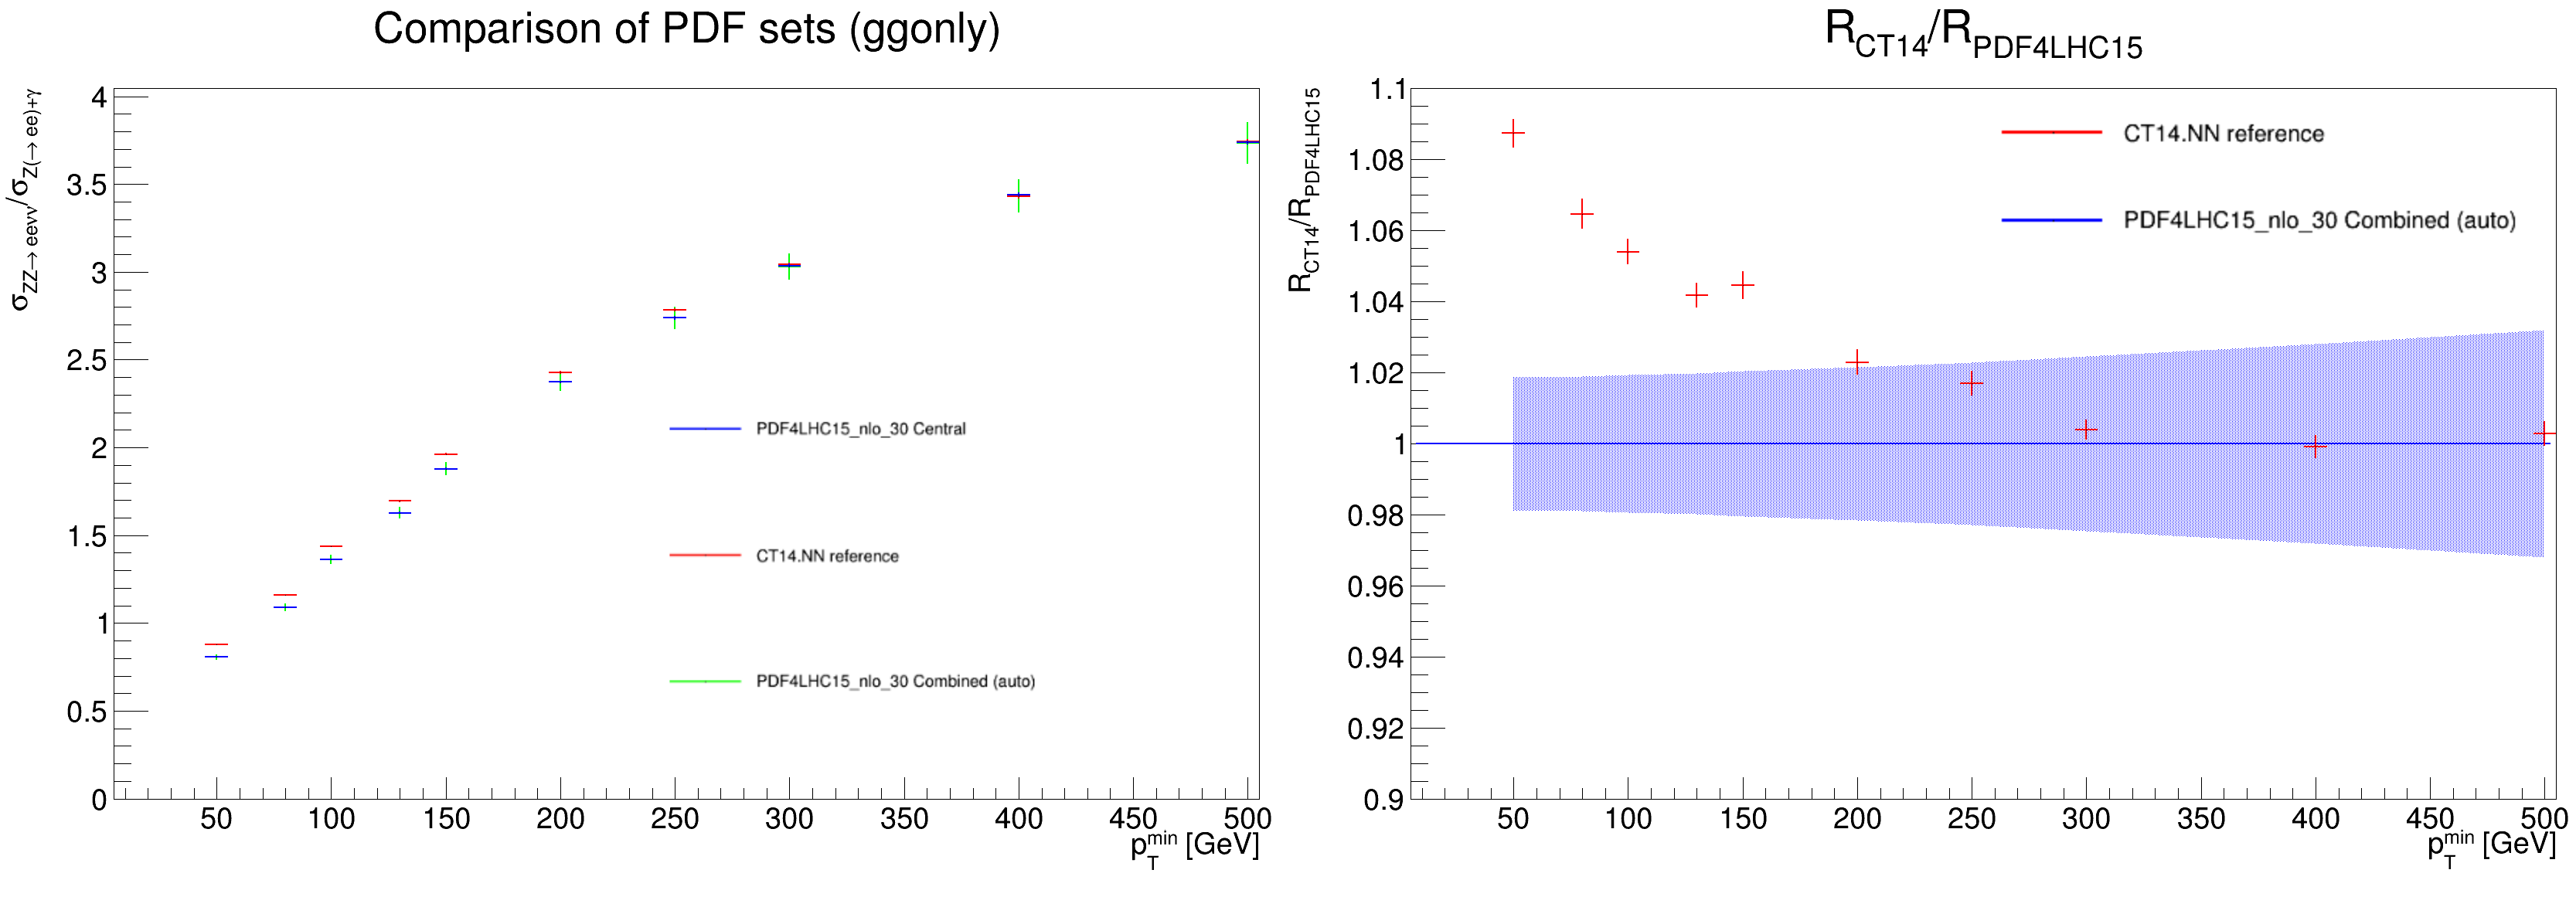
\includegraphics[width=\textwidth]{gg_PDF4.png}
%	\caption{$R_{gg}$ distribution from only the $gg$ contribution to the cross sections of $ZZ$ and $Z+\gamma$, using the combined uncertainties of \texttt{PDF4LHC15\_nlo\_30} sets. The figure on the right shows the ratio of the \texttt{CT14} set to the \texttt{PDF4LHC15\_nlo\_30} set.}
%	\label{pdfcompare_gg}
%\end{figure}
%The $gg$ contributions differ by a factor of 10. This curve appears to reach an a constant value at a higher $p_T$ value than the ratio curve constructed from the total cross section. The gluon gluon process is of interest, thus it has also been compared to the reference \texttt{CT14} set.

\subsection{Uncertainty from Photon Fragmentation}
The \Zgam process may contain photons that arise from the hadron showers. It is therefore important to isolate the prompt photon from hadronic activity. This reduces unwanted background from pion decays, or fragmentation processes.

Experimentally, photon isolation is implemented with the following cuts:
\begin{equation}
\sum_{\in R_0} E_T(\text{had}) < \epsilon_h p_T^\gamma \text{\hspace{1cm} or \hspace{1cm}} \sum_{\in R_0} E_T(\text{had}) < E_T^{max}
\end{equation}
\label{eq:photon_isol}
limiting the transverse hadronic energy $E_T(had)$ in a cone of size $R_0 = \sqrt{\Delta\eta^2 + \Delta\phi^2}$ around the photon, to some fraction of the photon $p_T$, or some fixed small cut-off.

The smooth cone isolation method of Frixione \cite{frixione} is an alternative isolation procedure, which simplifies calculations by avoiding fragmentation contribuitions. The following isolation prescription is applied to the photon:
\begin{equation}
	\sum_{R_{j\gamma} \in R_0} E_T(\text{had}) < \epsilon_h p_T^\gamma \left(\frac{1-\cos R_{j\gamma}}{1-\cos R_0}\right)^n.
\end{equation}
\label{eq:frix_isol}
where $R_{j\gamma}$ is the separation of the photon and the $j^{th}$ hadron. This requirement constrains the sum of hadronic energy inside a cone of radius $R_{j\gamma}$, for all separations $R_{j\gamma}$ less than a chosen cone size $R_0$. This prescription allows soft radiation inside the photon cone, but collinear singularities are removed. The smooth cone isolation is infrared finite, thus fragmentation contributions do not need to be included.\\
The relative isolation, given by Equation \ref{eq:photon_isol} is used in experimental analyses, while smooth isolation is difficult to implement experimentally. However, comparing both methods gives us an estimate of the uncertainty due to the modelling of photon fragmentation.

In this analysis, $R_0$ is chosen to be 0.4 to agree with the experimental definition. The central value is chosen to be from the sample using smooth cone isolation (Frixione) with $\epsilon_h = 0.075$ and $n=1$. These parameters are varied within a reasonable range to assess the uncertainty as shown in Figure \ref{fig:photon_frag}.

\begin{figure}[H]
\centering
	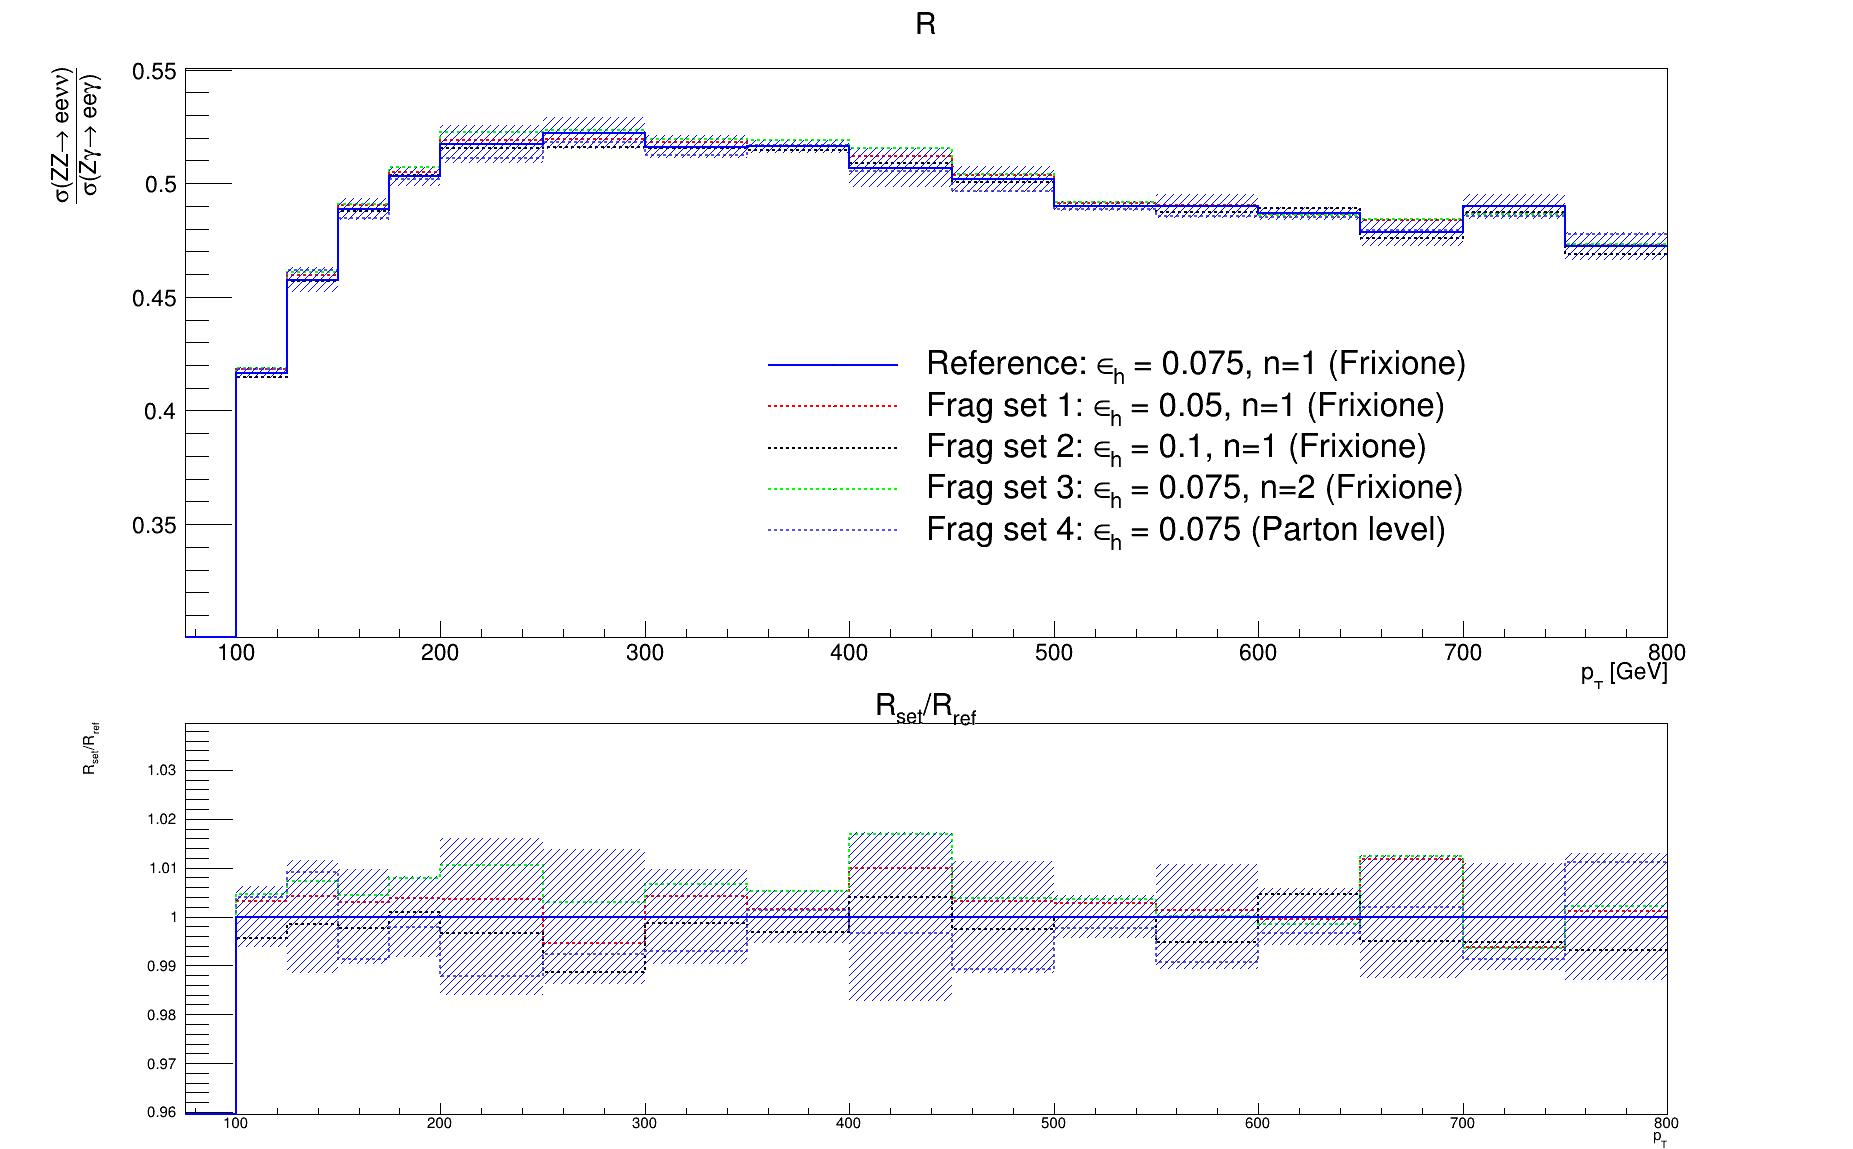
\includegraphics[width=\textwidth]{frag.png}
	\caption{$R$ distribution as a function of $p_T$, showing the uncertainty due to variation of photon isolation parameters $\epsilon_h$ and $n$ in the smooth cone isolation procedure (Frixione), and $\epsilon_h$ in the photon isolation procedure. The lower panel shows the relative deviation of the varied sets from the central value, as well as the uncertainty band.}
	\label{fig:photon_frag}
\end{figure}

The uncertainty is calculated from the four sets listed in Figure \ref{fig:photon_frag}:
\begin{equation}
\begin{split}
\delta R_i &= |R_i - R_{ref}| \hspace{2cm}  i \in (1,2,3,4)\\
\delta R &= \sqrt{\max_{i=1,2,3}(\delta R_i)^2 + (\delta R_4)^2}
\end{split}
\end{equation}
as the effects assessed by changing the isolation definition in set 4, and varying the parameters in sets 1-3 are different.\\
The uncertainty is $< 2\%$ over the whole range, which has been extended up till 800 GeV.

\section{Conclusion}
We propose a new method to estimate the \ZZ contribution to the $ll + E_T^{miss}$ signal from \Zgam data, using a transfer factor $R$, determined by simulation. We quantify the uncertainty from sources such as renormalization and factorization scales and different PDF distributions.\\From these, we observe that at high $p_T$, the value of $R$ approaches $0.47$, while at $p_T = 100$ GeV, $R = 0.40$. The uncertainty is quantified $\approx 2\%$ from scale variation, and $\approx 2.55\%$ from PDF variation. The uncertainty due to photon fragmentation is $<2\%$ for the full $p_T$ range, up to 800 GeV.

\section*{Acknowlegements}
This work was conducted under the patient supervision of Dr. Beate Heinemann. In addition to her guidance and advice, I had the help of Dr. Yee Chinn Yapp, who helped me work on streamlining the presentation of this work; Dr. Pieter Everaerts, who helped me debug the code and understand the physics better, and Dr. Sarah Heim, whose office is close enough to mine that I could bother her for the tiniest of details.

\begin{thebibliography}{9}

\bibitem{ZH_ATLAS}
	\textit{Search for an invisibly decaying Higgs boson or dark matter candidates produced in association with a Z boson in pp collisions at $\sqrt{s}$ = 13 TeV with the ATLAS detector}\\
	\textbf{ATLAS Collaboration}\\
	\texttt{arXiv:1708.09624}
	
\bibitem{gammajet}
	\textit{Using $\gamma +$ jets to calibrate the Standard Model $Z(\rightarrow \nu\nu)+$ jets background to new processes at the LHC}\\
	\textbf{S. Ask, M. A. Parker, T. Sandoval, M. E. Shea, W. J. Stirling}\\
Cavendish Laboratory, University of Cambridge, CB3 0HE, UK; 2011\\
	\texttt{[arXiv:1107.2803]}

\bibitem{Z_coupling}
	\textit{2017 Review of Particle Physics - Particle Listings}\\
	\textbf{C. Patrignani \textit{et al}. (Particle Data Group)}\\
	Chin. Phys. C, 40, 100001 (2016)
	
\bibitem{MCFM}
	\textit{Monte Carlo for FeMtobarn processes (MCFM) v8.0 User Manual}\\
	\textbf{John Campbell, Keith Ellis, Walter Giele, Ciaran Williams}\\
	\texttt{https://mcfm.fnal.gov/}
	
\bibitem{CT14}
	\textit{New parton distribution functions from a global analysis of quantum chromodynamics}\\
	\textbf{Sayipjamal Dulat, Tie Jiun Hou, Jun Gao, Marco Guzzi, Joey Huston, P. Nadolsky, Jon Pumplin, Carl Schmidt, Daniel Stump, C. P. Yuan}\\
	\texttt{arXiv:1506.07443}

\bibitem{PDF4}
	\textit{PDF4LHC recommendations for LHC Run II}\\
	\texttt{[arXiv:1510.03865]}	
	
\bibitem{MMHT14}
	\textit{Parton distributions in the LHC era: MMHT 2014 PDFs}\\
	\textbf{L. A. Harland-Lang, A. D. Martin, P. Motylinski, R. S. Thorne}\\
	\texttt{arXiv:1412.3989}
	
\bibitem{NNPDF3}
	\textit{Parton distributions for the LHC Run II}\\
	\textbf{The NNPDF Collaboration: Richard D. Ball, Valerio Bertone, Stefano Carrazza, Christopher S. Deans, Luigi Del Debbio, Stefano Forte, Alberto Guffanti, Nathan P. Hartland, Jose I. Latorre, Juan Rojo, Maria Ubiali}\\
	\texttt{arXiv:1410.8849}
	
\bibitem{LHAPDF}
	\textit{LHAPDF6: parton density access in the LHC precision era}\\
	\textbf{Andy Buckley, James Ferrando, Stephen Lloyd, Karl Nordstrom, Ben Page, Martin Ruefenacht, Marek Schoenherr, Graeme Watt}\\
	\texttt{arXiv:1412.7420}

\bibitem{frixione}
	\textit{Isolated photons in perturbative QCD}\\	
	\textbf{S. Frixione}\\
	Phys. Lett.B429(1998)369–374, hep-ph/9801442

\bibitem{ATHENA}
	\textit{ATHENA reference}\\
	\texttt{ATHENA reference}
	
\bibitem{powheg}
	POWHEG BOX - ZZ,WZ and WW production
	\begin{itemize}
	\item \textbf{P. Nason}\\
	JHEP 0411 (2004) 040, hep-ph/0409146
	\item \textbf{S. Frixione, P. Nason and C. Oleari}\\
	JHEP 0711 (2007) 070, \texttt{arXiv:0709.2092}
	\item \textbf{S. Alioli, P. Nason, C. Oleari and E. Re}\\
	JHEP 1006 (2010) 043, \texttt{arXiv:1002.2581}
	\item \textit{ZZ, WZ and W+W- production, including Gamma/Z interference, singly resonant contributions and interference for identical leptons}\\
	\textbf{T. Melia, P. Nason, R. Rontsch, G. Zanderighi}\\
	JHEP 1111 (2011) 078, \texttt{arXiv:1107.5051}
	\item \textit{W+W-, WZ and ZZ production in the POWHEG-BOX-V2}\\
	\textbf{P. Nason and G. Zanderighi}\\
	Eur.Phys.J. C74 (2014) 2702, \texttt{arXiv:1311.1365}
	\end{itemize}
	
\bibitem{pythia}
	\textit{PYTHIA 8.1}\\
	\textbf{T. Sjöstrand, S. Mrenna and P. Skands}\\
	JHEP05 (2006) 026, Comput. Phys. Comm. 178 (2008) 852. 
	
\bibitem{CT10}
	\textit{New parton distributions for collider physics}
	\textbf{Hung-Liang Lai, Marco Guzzi, Joey Huston, Zhao Li, Pavel M. Nadolsky, Jon Pumplin, C.-P. Yuan}
	\texttt{arXiv:1007.2241}
	
\bibitem{MSTW2008}
	\textit{Parton distributions for the LHC}\\
	\textbf{A.D. Martin, W.J. Stirling, R.S. Thorne, G. Watt}
	\texttt{arXiv:0901.0002}
	
\end{thebibliography}

\end{document}
